\chapter{PUMA - der digitale Zettelkasten}
\textit{Publikationen und Lesezeichen sammeln, verwalten und teilen, mit PUMA ein Kinderspiel.}\newline
\newline
Das Akademische Publikationsmanagement\index{Akademische 
Publikationsmanagement} (PUMA) ist ein System zum Sammeln, Verwalten, Teilen 
und Entdecken von Lesezeichen und Publikationen.\newline
Es ist zu vergleichen mit einem riesigen digitalen 
Zettelkasten, der für alle möglichen Quellen und Medien einsetzbar ist. PUMA 
ermöglicht Struktur und Ordnung für gesammelte Publikationen. Gespeicherte 
Publikationen und Lesezeichen lassen sich schnell wieder finden. Gleichzeitig 
bietet PUMA Platz für Notizen und Anmerkungen sowie eine Zusammenarbeit mit 
anderen PUMA-Nutzern. 
Die Software steht lizenzfrei als Webanwendung zur Verfügung.
\newline 
PUMA ist so konzipiert, dass es als alleiniges Eingabeportal für bibliografische Metadaten dienen kann. Außerdem können zu Literatureinträgen Dokumente hochgeladen werden. \newline
Durch die Vielzahl an Exportformaten und Schnittstellen zu anderen Programmen müssen die Nutzer ihre Daten nur einmal pflegen und können sie in anderen Systemen nachnutzen. Die wiederholte manuelle Eingabe von Publikationslisten entfällt. So können Forscher ihre Publikationslisten direkt aus PUMA auf ihre Homepage laden.  
\section{Für wen ist dieses Buch?} 
Dieses Buch richtet sich an die Angehörigen der Universität Stuttgart.
Die im Buch erklärten Beispiele basieren auf der PUMA-Installation der 
Universität. Diese Beispiele gelten in leicht abgewandelter 
Version für jede Institution, die PUMA installiert hat. 
\newline
Externe, die nicht der Universität Stuttgart angehören, können sich nicht bei 
dem hier vorgestellten PUMA anmelden. Für sie bietet sich die Nutzung 
von BibSonomy an. Da PUMA und BibSonomy über fast die gleichen Funktionen und 
Möglichkeiten verfügen, lassen sich die Beispiele aus dem Buch mit leichten 
Abweichungen auch auf BibSonomy übertragen.\newline
Besonders geeignet ist PUMA für
\begin{itemize}
\item Forschende, die ihre eigenen Publikationslisten verwalten.
\item Mitarbeitende, die Publikationslisten von Projekten, 
Instituten oder Fakultäten pflegen.
\item Studierende, die Material für Examensarbeiten verwalten 
möchten.
\item Autorinnen und Autoren, die ihre Veröffentlichungen der Unibibliografie 
melden möchten.
\item Studierende sowie Wissenschaftlerinnen und Wissenschaftler, 
die in Arbeitsgruppen Literatur teilen möchten.
\end{itemize}
\section{Typische Anwendungsbeispiele für PUMA}
PUMA ist für die Nutzung im akademischen Bereich entwickelt worden.
Es hilft bei Literaturrecherchen für eine Haus-, Bachelor- oder Masterarbeit, 
indem die recherchierte Literatur in PUMA gespeichert werden kann. Webseiten und 
Publikationen können mittels einer Schaltfläche (Bookmarklet) im Browser direkt 
in PUMA abspeichert werden. Am Ende der Arbeit hilft PUMA dabei das 
Literaturverzeichnis zu erstellen. Bei der Erstellung des Verzeichnisses kann 
aus 7.500 Zitationsstilen der passende ausgewählt werden oder auch eine 
individuelle Anpassung per Citation Style Language (CSL) vorgenommen werden.
\newline 
Eigene Veröffentlichungen können mit Hilfe von PUMA gepflegt und  durch den Tag 
\enquote{myown} gekennzeichnet werden. Dies vereinfacht das Erstellen einer 
Publikationsliste der eigenen Veröffentlichungen. Mit Hilfe des 
OpenCMS-Plugins kann die Publikationsliste direkt zum Beispiel auf der eigenen 
Homepage veröffentlicht werden und ist so für alle sichtbar.
\newline 
Ein weiteres typisches Anwendungsfeld bilden Institutspublikationslisten. 
Durch Erstellen einer Gruppe in PUMA kann eine gemeinsame Sammlung von 
Publikationen angelegt werden. Mit Hilfe des Plugins 
\enquote{Publikationsliste (aus BibSonomy/PUMA)} \index{Plugin für 
OpenCMS} kann eine Publikationsliste aus dieser 
Sammlung erzeugt werden.

   
\section{Anmelden\index{Anmeldung} bei PUMA} 
\begin{figure}[h!]
 \centering
 \fbox{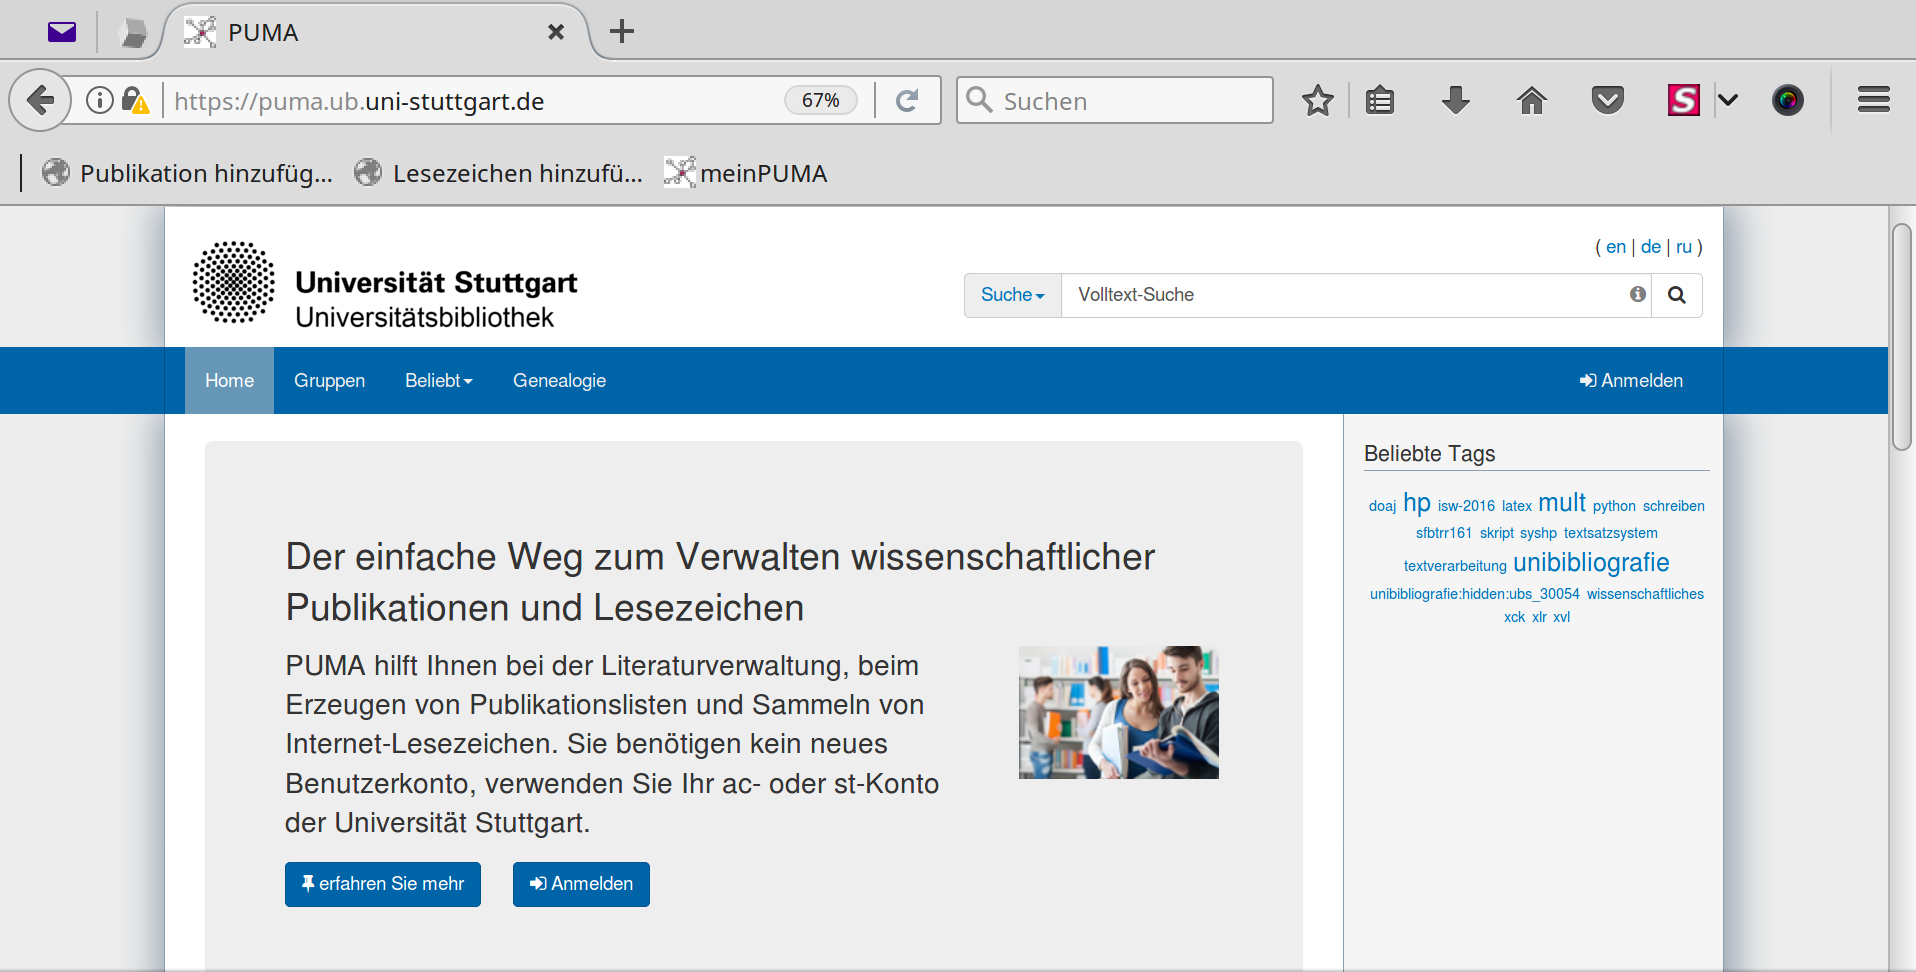
\includegraphics[width=10cm]{Bilder/Kapitel1/Startseite_PUMA}}
 \caption{Startseite PUMA}
 \label{figure001}
\end{figure}
\textbf{Vorab:} Sie benötigen ein st-, fn- oder ac-Konto der Universität Stuttgart.
\begin{enumerate}
    \item Rufen Sie die Anmeldeseite von PUMA auf:\newline \url{https://puma.ub.uni-stuttgart.de/}
    \item Geben Sie unter \enquote{Benutzername} Ihr ac- oder st-Konto der Universität Stuttgart ein (seltener ist das fn-Konto). 
    \item Unter  \enquote{Login} geben Sie Ihr Passwort ein. 
 \begin{figure}[h!]
 \centering
 \fbox{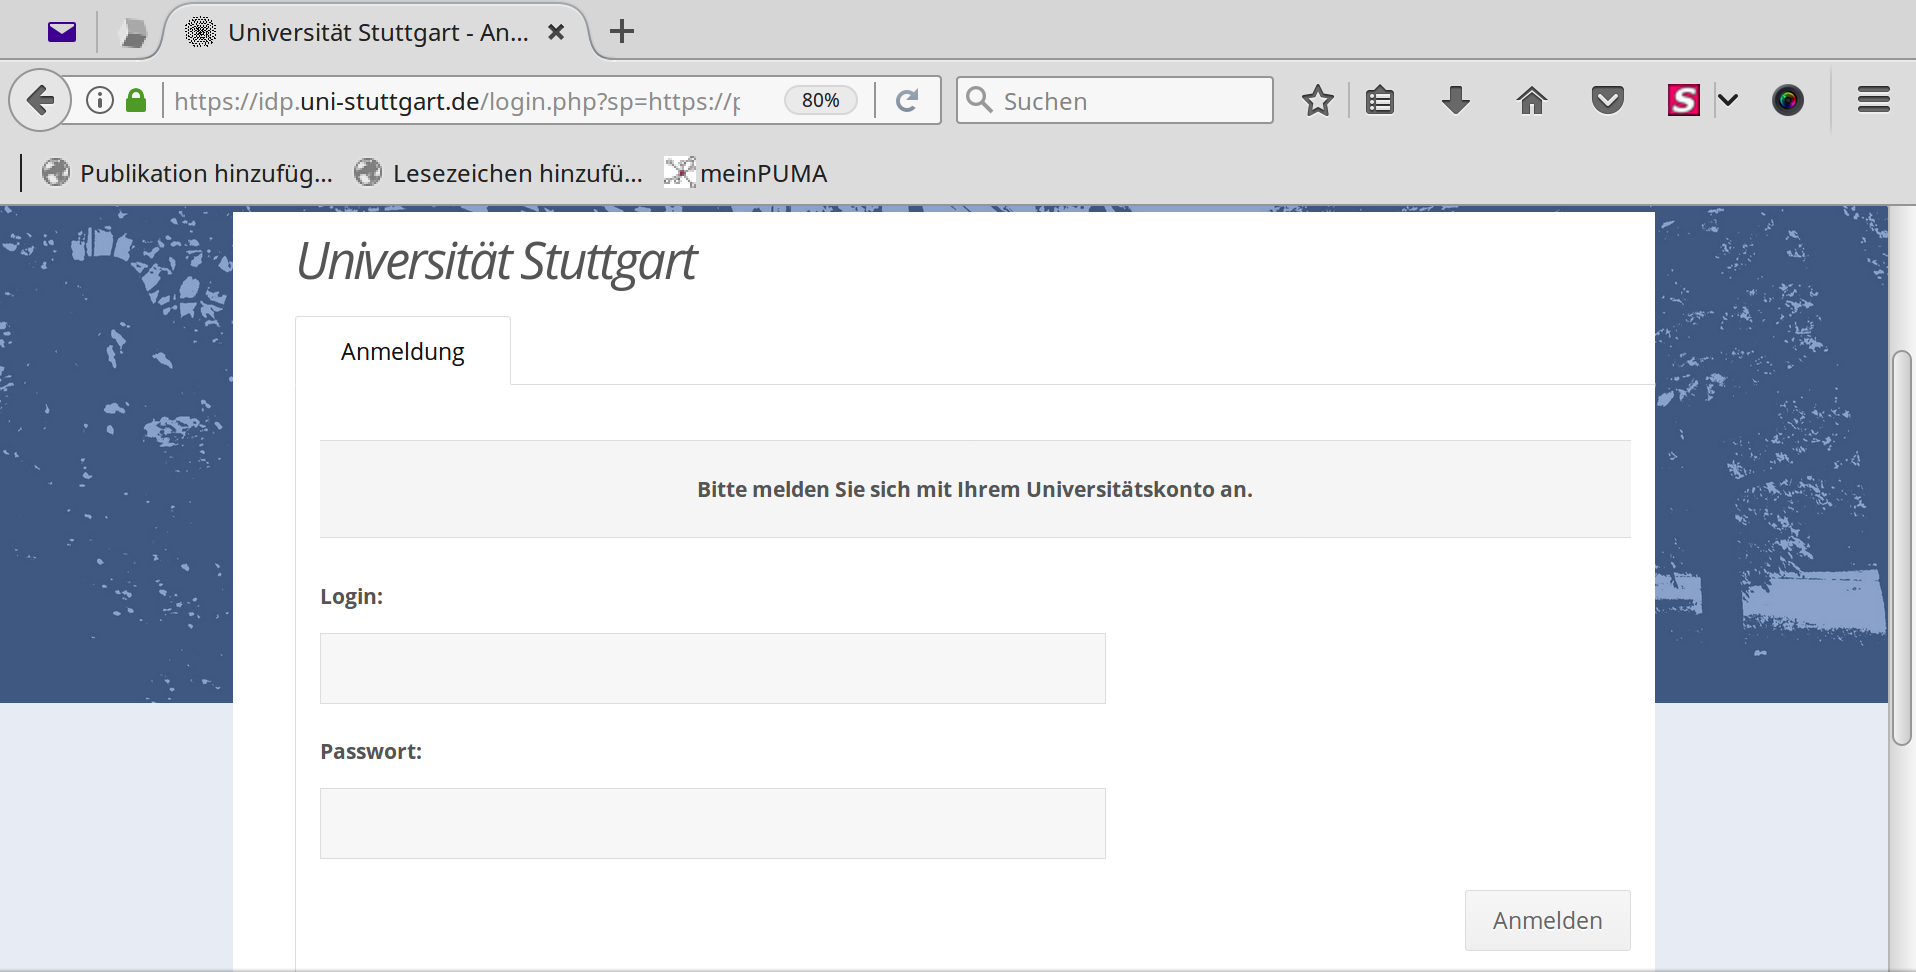
\includegraphics[width=9cm]{Bilder/Kapitel1/Anmeldung_bei_PUMA}}
 \caption{Anmeldung bei PUMA}
 \label{figure002}
\end{figure}  
    \item Klicken Sie auf \enquote{Anmelden}.
    \item Wenn Ihre Anmeldung erfolgreich war, zeigt Ihnen PUMA Ihre persönlichen Daten an. Überprüfen Sie die vorliegenden Daten, vergeben Sie einen Benutzernamen und klicken Sie anschließend auf \enquote{Registrieren}.
\end{enumerate}
Die Registrierung bei PUMA war erfolgreich. Ab sofort können Sie sich bei PUMA mit Ihrem Benutzerkonto anmelden. \newline
Bei der erstmaligen Anmeldung ist die Vergabe eines Benutzernamens erforderlich. Nur bei öffentlich geteilten Einträgen erscheint er bei den Publiaktionseinträgen in der Form @benutzername.
\section{Der PUMA-Blog}
Im Blog der Universitätsbibliothek Stuttgart (UB) ist neben allgemeinen Informationen zu der UB auch die Kategorie \enquote{PUMA} an wählbar (\url{http://blog.ub.uni-stuttgart.de/category/puma/}). Hier können die Nutzer sich über die aktuellen PUMA-Ereignisse einen Überblick verschaffen und werden über PUMA-Updates und neue Funktionen informiert.\newline
Mit Hilfe eines RSS-Feeds können Interessierte Informationen zu Server-Updates abonnieren. Über den Link: \url{http://blog.ub.uni-stuttgart.de/category/puma/feed/} werden die aktuellen Informationen angezeigt. Durch das Klicken auf \enquote{Jetzt abonnieren} öffnet sich ein Fenster, indem das Abonnieren nochmals bestätigt werden muss. Ab sofort können die Informationen über die Lesezeichen-Leiste angezeigt werden. 
\section{BibSonomy\index{BibSonomy}}
PUMA steht nur den Mitgliedern der Universität Stuttgart zu Verfügung, die über ein st-, fn- oder ac-Konto  verfügen. Für externe Nutzer der Universitätsbibliothek Stuttgart besteht die Möglichkeit das Muttersystem von PUMA, BibSonomy, zu nutzen. Beide Systeme verfügen über fast die gleichen Funktionen und Möglichkeiten seine Publikationen und Lesezeichen zu sammeln, verwalten und teilen. \newline
Die Anmeldung bei BibSonomy erfolgt über die Homepage \newline
\url{http://www.bibsonomy.org/?lang=de}.  

%\section{BibSonomy\index{BibSonomy} vs. PUMA}
%\suppressfloats[t]
\begin{table}[h!]
\tabulinesep=1.5mm
\begin{tabu}{|X[1.4,c]|X[2.2,m]|X[2,m]|} 
\tabucline[0.5pt]-\everyrow{\tabucline[0.5pt]-} 
\rowfont\bfseries
Unterschiede & PUMA \emph{Uni Stuttgart} & BibSonomy\\ \tabucline[1pt]-
\bfseries{Anmeldung}\strut & Nur möglich mit einem st-, fn- oder ac-Konto der Universität, mit dem sich die Nutzer authentifizieren.  & Für jeden frei zugänglich, ein Benutzerkonto muss selber angelegt werden. \\ 
\bfseries{Gruppen}\index{Gruppen} & Gruppen können jederzeit und selbständig gegründet werden. & Die Gründung einer Gruppe erfordert die Freigabe des BibSonomy-Admins. \\
\bfseries{OPUS}\index{OPUS} & Für die Zukunft geplant. Ermöglicht den Nutzern ein direktes Veröffentlichen auf dem Dokumentenserver OPUS. & \\ 
\bfseries{Unibibliografie}\index{Unibibliografie}& Die Publikationsmetadaten der Unibibliografie stehen zum Beispiel für Institutspublikationslisten zur Nachnutzung zur Verfügung.&\everyrow{} \\ \tabucline[1.0pt]-
\end{tabu}
\caption{Unterschiede zwischen PUMA und BibSonomy}
\end{table}
%\normalsize